% Standalone TikZ figure: Successive Halving and Multi-Fidelity Optimization
% For Chapter 2: Background and Theoretical Foundations
\documentclass[tikz,border=10pt]{standalone}
\usepackage{tikz}
\usetikzlibrary{arrows.meta, positioning, shapes.geometric, fit, backgrounds, calc, decorations.pathreplacing}

\begin{document}
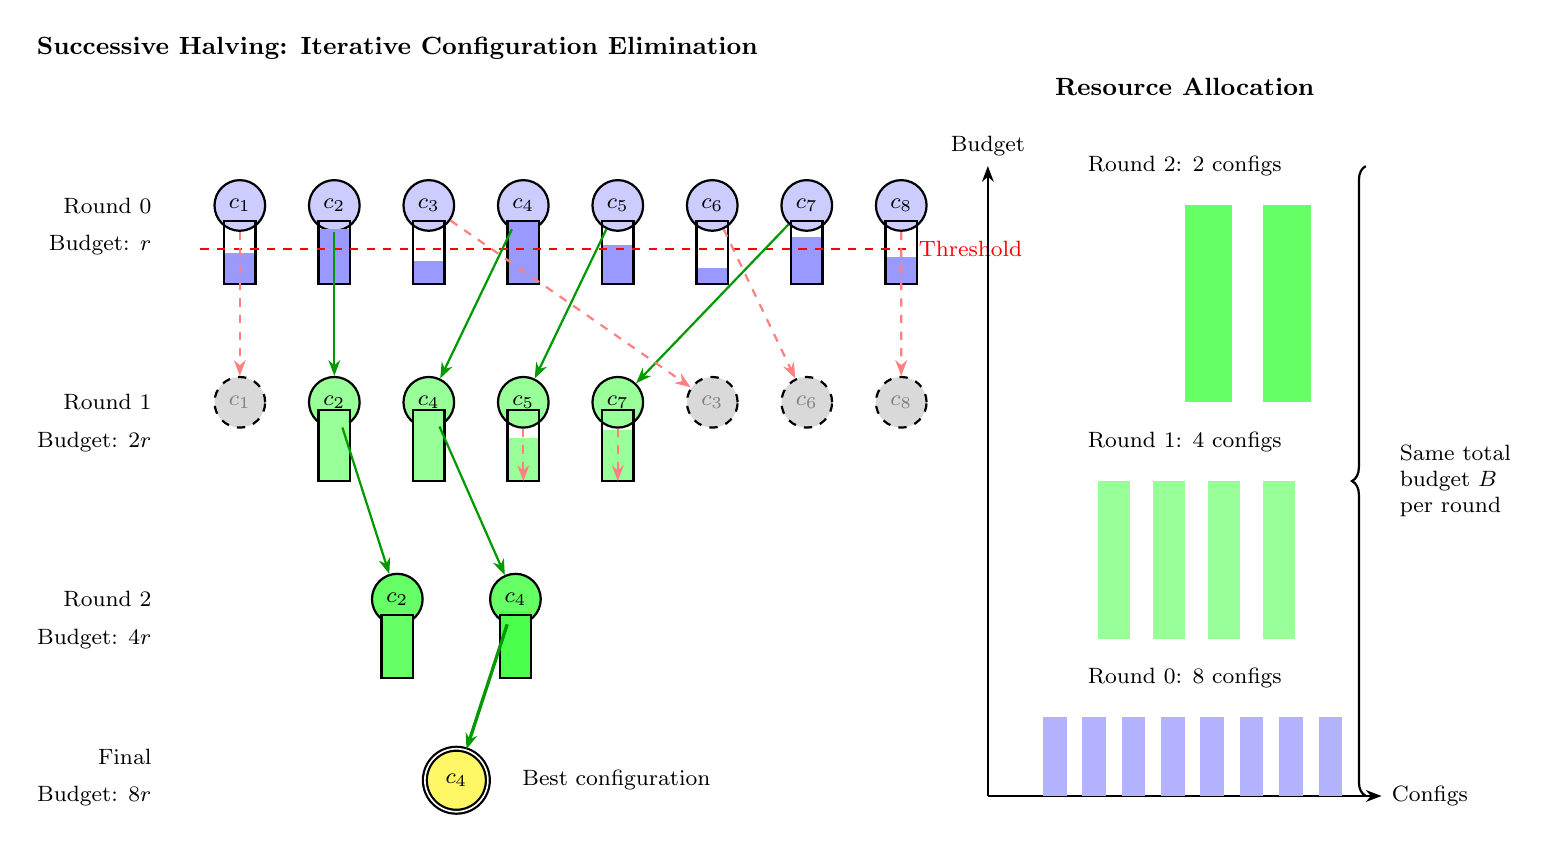
\begin{tikzpicture}[
    node distance=0.5cm and 0.8cm,
    every node/.style={font=\small},
    config/.style={circle, draw, thick, minimum size=0.6cm},
    goodconfig/.style={circle, draw, thick, minimum size=0.6cm, fill=green!40},
    badconfig/.style={circle, draw, thick, minimum size=0.6cm, fill=red!30},
    elimconfig/.style={circle, draw, thick, minimum size=0.6cm, fill=gray!30, dashed},
    arrow/.style={-{Stealth[length=2mm]}, thick},
    label/.style={font=\footnotesize},
    title/.style={font=\bfseries\small}
]

% Title
\node[title] at (0, 2) {Successive Halving: Iterative Configuration Elimination};

% ============ ROUND 0: All configurations ============
\node[label, left] at (-3, 0) {Round 0};
\node[label, left] at (-3, -0.5) {Budget: $r$};

% 8 configurations
\foreach \i in {1,...,8} {
    \pgfmathsetmacro{\xpos}{-2 + (\i-1)*1.2}
    \node[config, fill=blue!20] (c0\i) at (\xpos, 0) {\footnotesize $c_\i$};
}

% Performance bars for round 0
\foreach \i/\h in {1/0.4, 2/0.7, 3/0.3, 4/0.8, 5/0.5, 6/0.2, 7/0.6, 8/0.35} {
    \pgfmathsetmacro{\xpos}{-2 + (\i-1)*1.2}
    \fill[blue!40] (\xpos-0.2, -1) rectangle (\xpos+0.2, -1+\h);
    \draw[thick] (\xpos-0.2, -1) rectangle (\xpos+0.2, -0.2);
}

% Threshold line
\draw[red, thick, dashed] (-2.5, -0.55) -- (6.5, -0.55);
\node[label, red, right] at (6.5, -0.55) {Threshold};

% ============ ROUND 1: Top 4 ============
\node[label, left] at (-3, -2.5) {Round 1};
\node[label, left] at (-3, -3) {Budget: $2r$};

% Surviving configurations (top 4: c2, c4, c5, c7)
\node[goodconfig] (c12) at (-0.8, -2.5) {\footnotesize $c_2$};
\node[goodconfig] (c14) at (0.4, -2.5) {\footnotesize $c_4$};
\node[goodconfig] (c15) at (1.6, -2.5) {\footnotesize $c_5$};
\node[goodconfig] (c17) at (2.8, -2.5) {\footnotesize $c_7$};

% Eliminated
\node[elimconfig] (e1) at (-2, -2.5) {\footnotesize \textcolor{gray}{$c_1$}};
\node[elimconfig] (e3) at (4, -2.5) {\footnotesize \textcolor{gray}{$c_3$}};
\node[elimconfig] (e6) at (5.2, -2.5) {\footnotesize \textcolor{gray}{$c_6$}};
\node[elimconfig] (e8) at (6.4, -2.5) {\footnotesize \textcolor{gray}{$c_8$}};

% Arrows showing survival
\draw[arrow, green!60!black] (c02) -- (c12);
\draw[arrow, green!60!black] (c04) -- (c14);
\draw[arrow, green!60!black] (c05) -- (c15);
\draw[arrow, green!60!black] (c07) -- (c17);

% Arrows showing elimination
\draw[arrow, red!50, dashed] (c01) -- (e1);
\draw[arrow, red!50, dashed] (c03) -- (e3);
\draw[arrow, red!50, dashed] (c06) -- (e6);
\draw[arrow, red!50, dashed] (c08) -- (e8);

% Performance bars for round 1
\foreach \i/\h/\xpos in {2/0.75/-0.8, 4/0.9/0.4, 5/0.55/1.6, 7/0.65/2.8} {
    \fill[green!40] (\xpos-0.2, -3.5) rectangle (\xpos+0.2, -3.5+\h);
    \draw[thick] (\xpos-0.2, -3.5) rectangle (\xpos+0.2, -2.6);
}

% ============ ROUND 2: Top 2 ============
\node[label, left] at (-3, -5) {Round 2};
\node[label, left] at (-3, -5.5) {Budget: $4r$};

% Surviving configurations (top 2: c2, c4)
\node[goodconfig, fill=green!60] (c22) at (0, -5) {\footnotesize $c_2$};
\node[goodconfig, fill=green!60] (c24) at (1.5, -5) {\footnotesize $c_4$};

% Arrows
\draw[arrow, green!60!black] (c12) -- (c22);
\draw[arrow, green!60!black] (c14) -- (c24);
\draw[arrow, red!50, dashed] (c15) -- ++(0, -1);
\draw[arrow, red!50, dashed] (c17) -- ++(0, -1);

% Final performance
\fill[green!60] (-0.2, -6) rectangle (0.2, -5.2);
\draw[thick] (-0.2, -6) rectangle (0.2, -5.2);
\fill[green!70] (1.3, -6) rectangle (1.7, -5.15);
\draw[thick] (1.3, -6) rectangle (1.7, -5.2);

% ============ FINAL: Best configuration ============
\node[label, left] at (-3, -7) {Final};
\node[label, left] at (-3, -7.5) {Budget: $8r$};

\node[goodconfig, fill=yellow!60, double, minimum size=0.8cm] (winner) at (0.75, -7.3) {\footnotesize $c_4$};
\draw[arrow, green!60!black, very thick] (c24) -- (winner);

\node[label, right=0.3cm of winner] {Best configuration};

% ============ RESOURCE ALLOCATION DIAGRAM (RIGHT SIDE) ============
\node[title] at (10, 1.5) {Resource Allocation};

% Axes
\draw[arrow] (7.5, -7.5) -- (7.5, 0.5) node[above, label] {Budget};
\draw[arrow] (7.5, -7.5) -- (12.5, -7.5) node[right, label] {Configs};

% Bars showing resource allocation
% Round 0: 8 configs, small budget each
\foreach \i in {1,...,8} {
    \fill[blue!30] (7.7+\i*0.5, -7.5) rectangle (8+\i*0.5, -6.5);
}
\node[label] at (10, -6) {Round 0: 8 configs};

% Round 1: 4 configs, medium budget
\foreach \i in {1,...,4} {
    \fill[green!40] (8.2+\i*0.7, -5.5) rectangle (8.6+\i*0.7, -3.5);
}
\node[label] at (10, -3) {Round 1: 4 configs};

% Round 2: 2 configs, large budget
\foreach \i in {1,...,2} {
    \fill[green!60] (9+\i*1, -2.5) rectangle (9.6+\i*1, 0);
}
\node[label] at (10, 0.5) {Round 2: 2 configs};

% Total budget annotation
\draw[decorate, decoration={brace, amplitude=5pt}, thick]
    (12.3, -7.5) -- (12.3, 0.5)
    node[midway, right=0.3cm, align=left, label] {
        Same total\\
        budget $B$\\
        per round
    };

\end{tikzpicture}
\end{document}
